% !TeX spellcheck = fr_FR
\chapter{Chapitre 1 : Analyse}

Ce chapitre a pour but d'expliquer de manière détaillée l'objectif de ce projet de semestre. Je vais aussi faire part des différentes idées qui sont ressorties lors de nos discussions avec mon professeur. Par la suite, je vais expliquer en quoi consiste la fonction de hachage Bcrypt, son fonctionnement et ses spécificités. Pour finir, je vais rapporter les différentes implémentations sur \gls{fpga} que j'ai pu retrouver et celui que j'ai fini par reprendre durant le projet de semestre. 

\section{Description du projet}

L'objectif principal de ce projet est d'exploiter le parallélisme offertes par les \gls{fpga}, afin de calculer les fonctions de hachage nécessitant beaucoup de temps de calculs. Le but étant d'avoir au final un système plus efficient que les solutions actuels lors d'une attaque par bruteforce. Il est aussi nécessaire d'avoir une certaine communication entre le \gls{pc} de l'attaquant et le \gls{fpga}, afin que l'attaquant puisse fournir le hash qu'il suite casser.

\begin{figure}[tbph!]
	\centering
	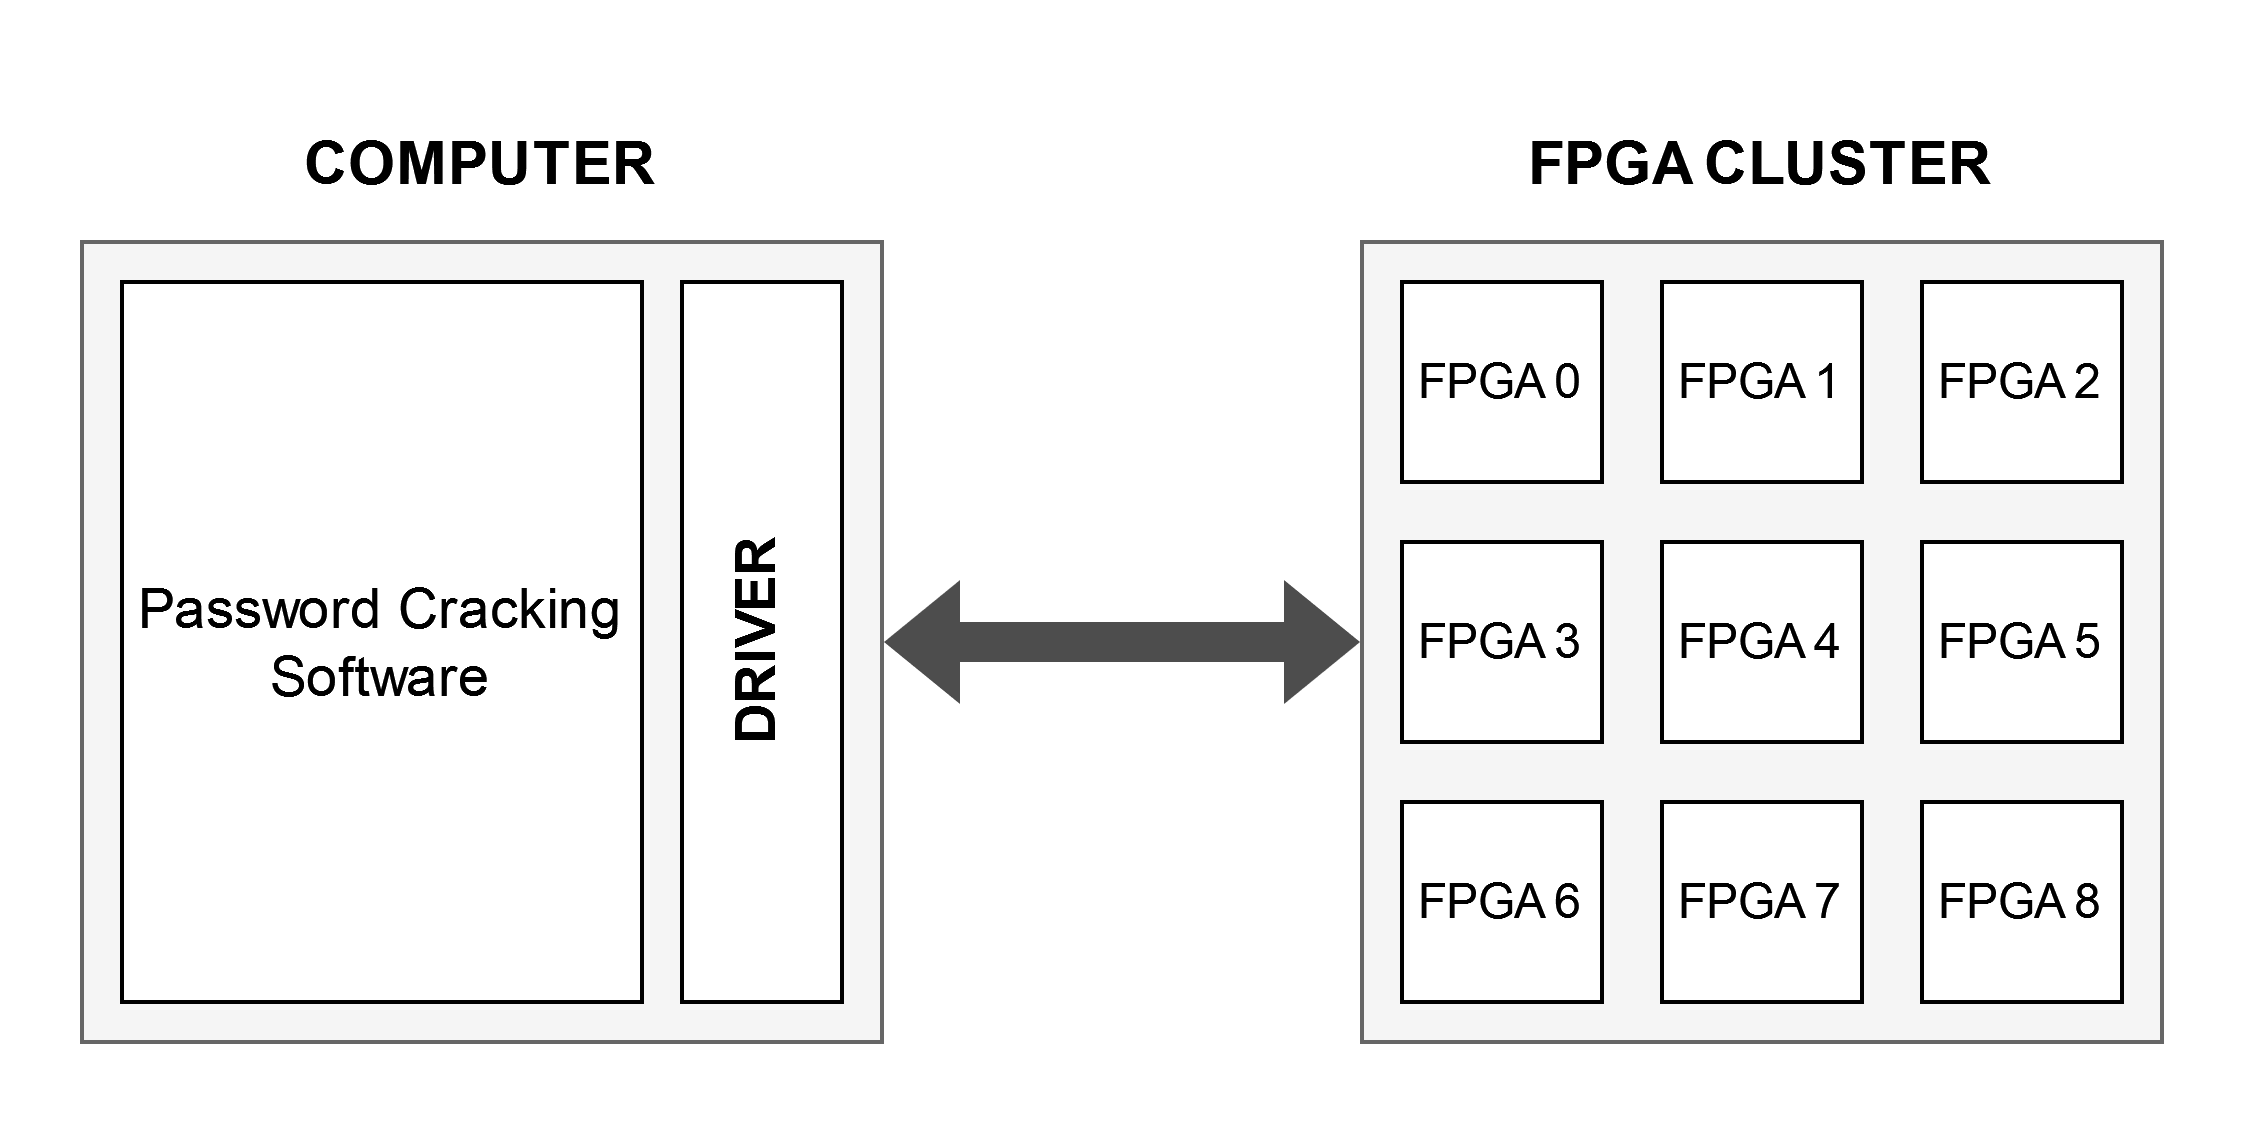
\includegraphics[width=0.7\linewidth]{objectif}
	\caption[Diagramme général]{Diagramme général. Source : réalisé par Kandiah Abivarman}
	\label{fig:objectif}
\end{figure}

Une des première questions qu'on s'était posé avec les professeurs était la manière de générer les mots de passes lors d'une attaque. Dans notre cas, nous avons deux possibilités, soit nous générons les mots de passes directement depuis le \gls{pc} et devons les transmettre à la carte\gls{fpga} afin de procéder au hachage 

\section{Bcrypt}

Votre texte, votre texte, votre texte, votre texte, votre texte, votre texte, votre texte, votre texte, votre texte, votre texte, votre texte, votre texte, votre texte, votre texte, votre texte, votre texte, votre texte, votre texte.

\begin{figure}[tbph!]
	\centering
	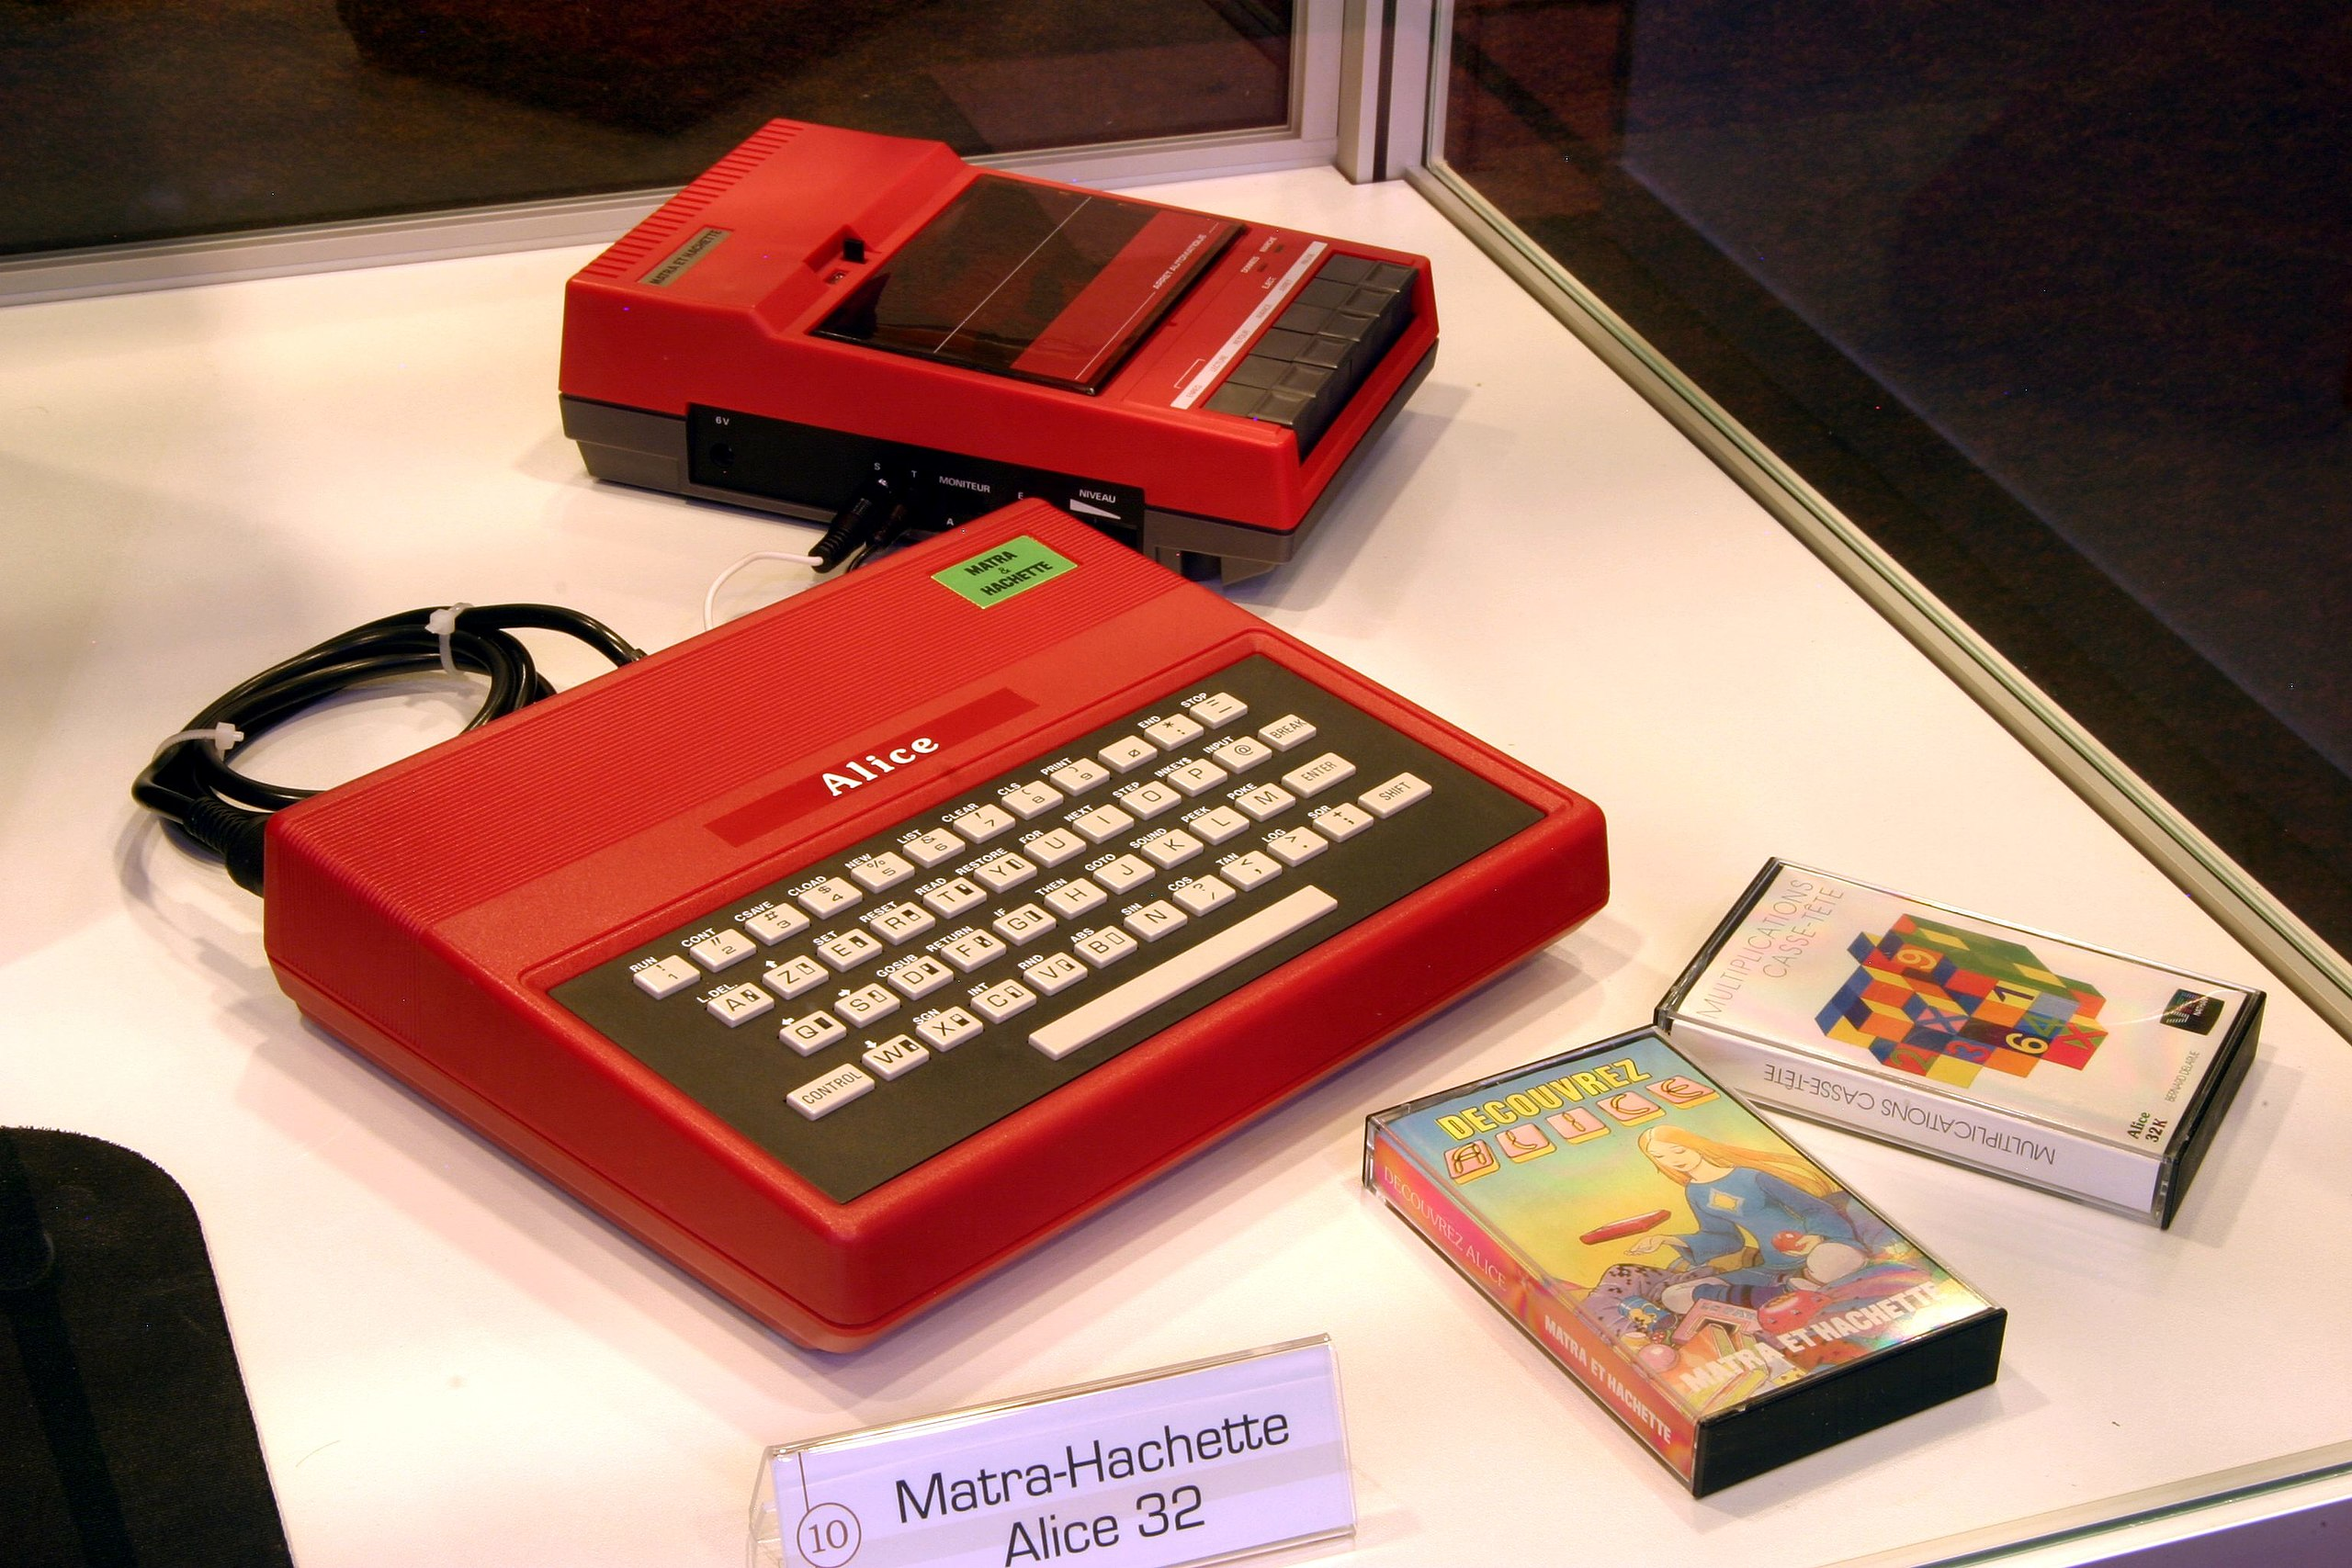
\includegraphics[width=0.7\linewidth]{ordi}
	\caption[Alice, Micro-ordinateur MATRA.]{Alice, Micro-ordinateur MATRA. Source : tiré de Tartempion 2010, p. 42 / tiré de ce-site.ch, ref. URL03 / réalisé par Nom Prénom.}
	\label{fig:image}
\end{figure}


\subsection{Algorithme}

Votre texte, votre texte, votre texte, votre texte, votre texte, votre texte, votre texte, votre texte, votre texte, votre texte, votre texte, votre texte, votre texte, votre texte, votre texte, votre texte, votre texte, votre texte.


\subsection{Format du Hash}

Votre texte, votre texte, votre texte, votre texte, votre texte, votre texte, votre texte, votre texte, votre texte, votre texte, votre texte, votre texte, votre texte, votre texte, votre texte, votre texte, votre texte, votre texte.

\begin{table}[tbph!]
	\centering{
		\begin{tabular}{ |l|c|c|c| }
			\hline
			& \textbf{Condition 1} & \textbf{Condition 2} & \textbf{Condition 3} \\
			\hline
			\textbf{Test 1} & X & O & X \\
			\hline
			\textbf{Test 2} & O & X & X \\
			\hline
			\textbf{Test 3} & O & X & O \\
			\hline 
		\end{tabular}
		\caption[Lot de données n°2.]{Lot de données n°2. Source: tiré de Tartempion 2010, p. 42 / tiré de ce-site.ch, ref. URL05 / réalisé par Nom Prénom.}
		\label{tab:tableau2}
	}
\end{table}

Votre texte, votre texte, votre texte, votre texte, votre texte, votre texte, votre texte, votre texte, votre texte, votre texte, votre texte, votre texte, votre texte, votre texte, votre texte, votre texte, votre texte, votre texte.

\section{Implémentations Existantes}